\section{Algorithm Specification}

\subsection*{\textit{Version 1.0}}

\subsection{Introduction}

The CIShell Platform has been specifically designed around the idea of the
algorithm. It is the central and most important concept. Algorithms are fully
defined and self-contained bits of execution. They can do many things from data
conversion, data analysis, and can even spawn whole outside programs if needs be.
Algorithms are very well defined black boxes in that what can come into and out
of the algorithm is specified in each algorithm's metadata. Other than that,
CIShell makes no attempt to understand the algorithm.

Figure \ref{fig:algExecWorkflow} shows the flow of information into and out of an
algorithm. Here an algorithm is passed zero or more pieces of data, any
user-entered parameters, and a CIShell context. The algorithm is then executed
and produces zero or more pieces of data.

\begin{figure}[htb!]
\centering
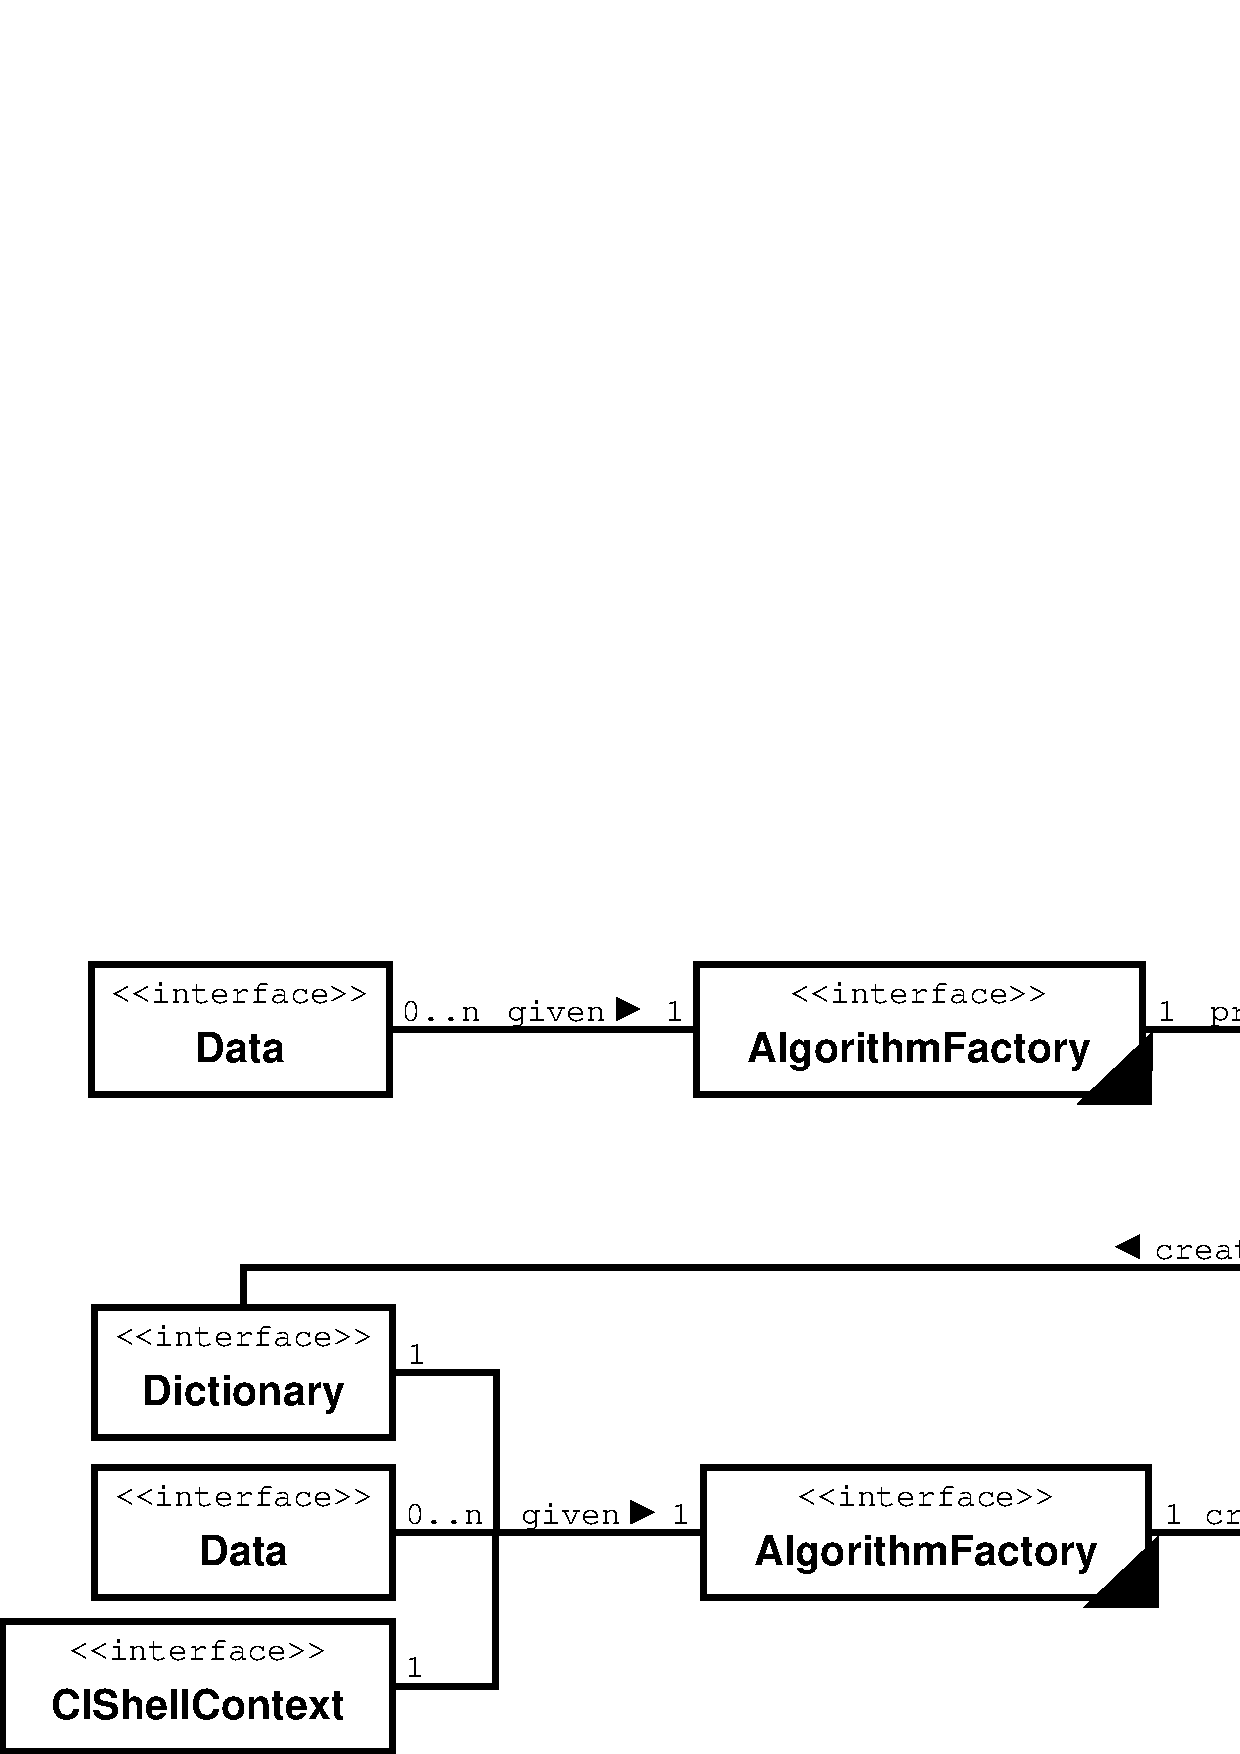
\includegraphics[width=150mm]{../img/algExecWorkflow.pdf}
\caption{Algorithm Execution Workflow}
\label{fig:algExecWorkflow}
\end{figure}

An algorithm defines its inputs in two ways. First, the input Data is defined
in the algorithm's service metadata. Second, the acceptable user-entered
parameters are defined in a MetaTypeProvider. This MetaTypeProvider defines the
types, value range, and textual description of the parameters needed. From this
information, a user interface (UI) can be created that asks a user for the
data.

\subsection{Standard Algorithm Properties}
\orgcishellframeworkalgorithm{}
